\chapter{Elementi Costitutivi}\label{Hardware}

\begin{minipage}{12cm}\textit{Se lo si desidera, utilizzare questo spazio per inserire un breve riassunto di ci\`o che verr\`a detto in questo capitolo. Inserire solo i punti salienti.}
\end{minipage}

\vspace*{1cm}


\section{Trasformatore - Modello di Tokamak}\label{Trasformatore}

La tesi va scritta usando la terza persona, per quanto possibile, tranne casi veramente eccezionale. In inglese \`e piuttosto standard usare la prima persona (plurale) in testi tecnici. In italiano no.

\subsection{Modellazione Fisica}
\subsection{Funzione di Trasferimento}

\newpage


\section{Sensore di Corrente}\label{CurrentSense}
Benché per gli obiettivi di controllo la lettura della corrente sul primario non è indispensabile, si è però preferito poter misurare cosa stia succedendo all'interno del sistema.\\

\subsection{Regime di funzionamento}
Per allo scopo di misurare la corrente è stato messo in serie al primario il sensore di Corrente \cite{ACS770}
Le scelte che hanno portato alla sua scelta sono: \vspace{-8mm}
\begin{center}
	\begin{tabular}[t]{|l r|}
		\hline
		Bandwidth:                             & 120 kHz                               \\
		Output rise time :                     & 4.1 $ \mu s $                         \\
		Ultralow power loss:                   & 100 $ \mu \Omega $ Resistenza Interna \\
		Single supply operation                & 4.5 to 5.5 V                          \\
		Extremely stable output offset voltage &                                       \\
		\hline
	\end{tabular}
\end{center}

\begin{figure}[h]
	\centering
	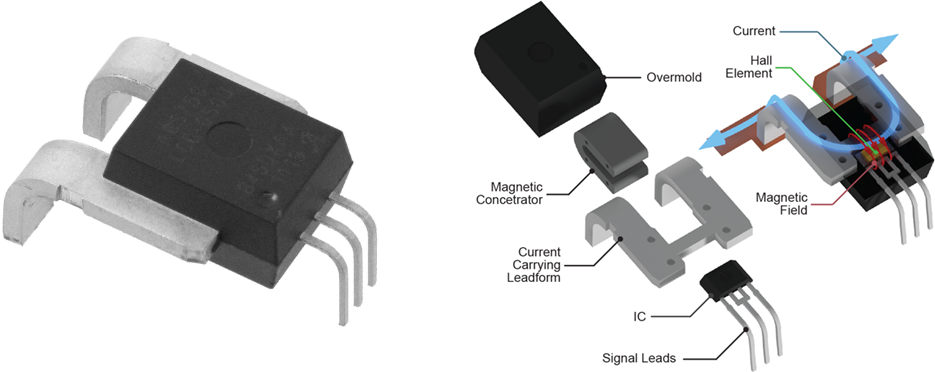
\includegraphics[width=1\textwidth]{ACS770/ACS770-Fig.png}
	\caption[Sensore di Corrente \citefield{ACS770}{series}]{Sensore di Corrente}
\end{figure}


\noindent
Delle tante varianti presenti, si è scelto di usare la \citefield{ACS770}{series}, le cui caratteristiche chiave di questa variante sono:
\begin{center}
	\begin{tabular}[t]{|l r|}
		\hline
		Primary Sampled Current: & $\pm$ 100 A     \\
		Sensitivity Sens (Typ.)  & 20(mV/A)        \\
		Current Directionality   & Bidirectional   \\
		$T_{OP}$                 & –40 to 150 (°C) \\
		\hline
	\end{tabular}
\end{center}

\noindent
Queste caratteristiche lo rendono adatto per misurare i nostri esperimenti comprendo tutti i possibili valori di corrente misurabili.\\
Essendo però il principio di funzionamento basato su un sensore a effetto Hall, ovvero una misura diretta del campo magnetico indotto, è importante tenere distante il sensore dal trasformatore che nei suoi momenti di massimo flusso, genera ovviamente un campo magnetico non indifferente.

\subsection{Funzionamento Interno}

Tra le caratteristiche chiave dell'\cite{ACS770}, troviamo il disaccoppiamento fisico tra la corrente da misurare e il circuito di misura, come è possibile vedere nel suo schema a blocchi: 

\begin{figure}[h]
	\centering
	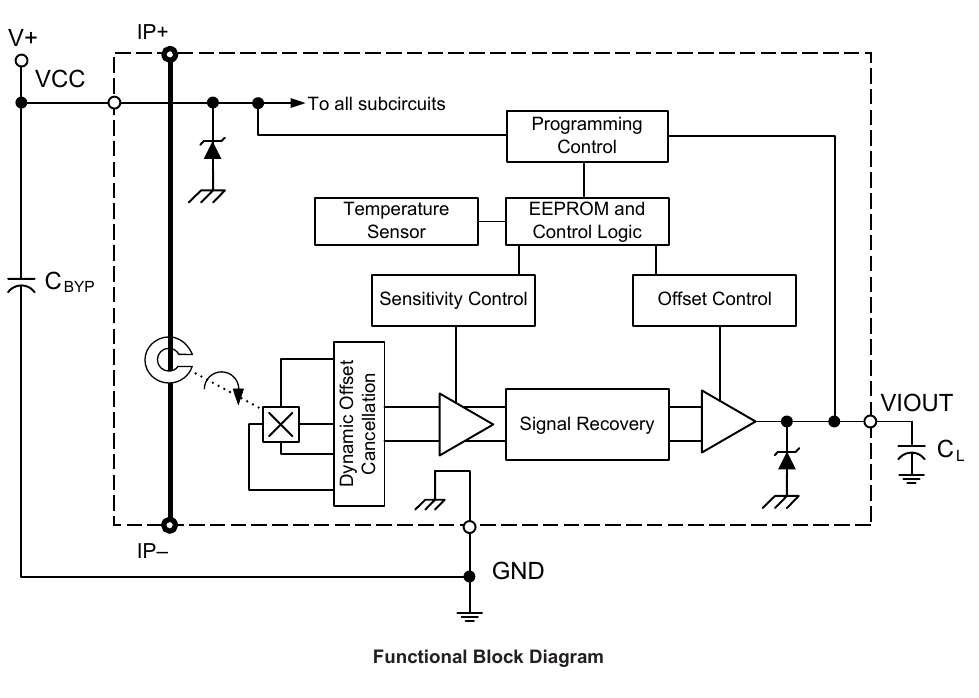
\includegraphics[width=1\textwidth]{ACS770/ACS770-SchemaBlocchi.png}
	\caption[\citefield{ACS770}{series} Schema a Blocchi]{Schema a Blocchi}
\end{figure}

\noindent
Questa caratteristica chiave, garantisce la salvaguardia del circuito logico a valle, dai possibili eventi catastrofici a monte.\\
Esso è in oltre fornito di sensori di temperatura e sistemi di "Signal Recovery" che permettono in Hardware di compensare derive termiche e \nonLinearita, ottenendo un output assimilabile a un segnale lineare:

\begin{figure}[h]
	\centering
	\includegraphics[width=0.6\textwidth]{ACS770/ACS770-Sensibilità.png}
	\caption[\citefield{ACS770}{series} Sensibilità rispetto Temperatura]{Sensibilità}
\end{figure}

\noindent
Esso ovviamente varia in base alla temperatura, e l'errore è tanto più marcato tanto maggiore è la corrente da misurare, ma leggendo dal datasheet abbiamo che questo errore, che dipende si dalle temperature di esercizio dell'esperimento, non è mai, neanche negli esperimenti più sfortunati, superiore al $\pm2\%$.\\
Anzi, alle temperature $\approx$ 25°, si mantiene contenuto tra $\pm0.5\%$.

\begin{figure}[h]
	\centering
	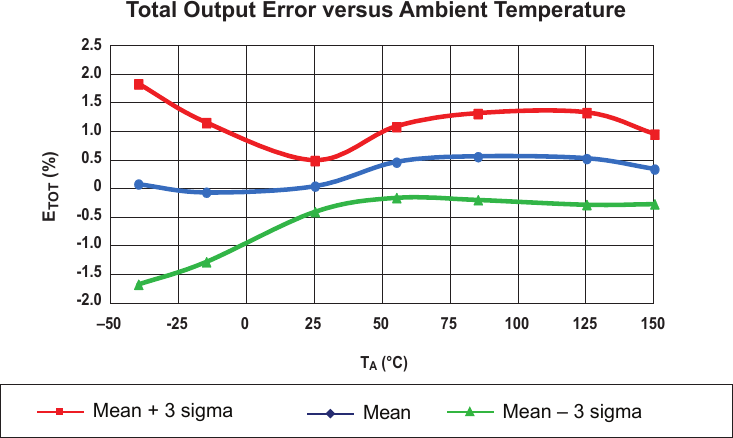
\includegraphics[width=0.55\textwidth]{ACS770/ACS770-NonLin.png}
	\caption[\citefield{ACS770}{series} \nonLinearita]{Temperatura/NonLinearità}
\end{figure}

\newpage

\subsection{Connessione elettrica}

La connessione del sensore è particolarmente semplice, richiedendo esternamente solo un alimentazione stabilizzata e portando subito in uscita la misura.
\begin{figure}[h]
	\centering
	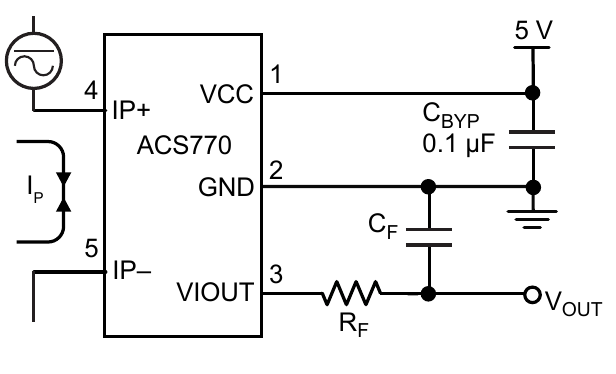
\includegraphics[width=1\textwidth]{ACS770/ACS770-Schema.png}
	\caption[\citefield{ACS770}{series} Schema di collegamento]{Schema di Collegamento}
\end{figure}

\noindent
Rispetto allo schema proposto dal datasheet, però, si è anche deciso di omettere il filtro passa-basso sulla \textbf{VIOUT}, questa scelta è stata presa per minimizzare il più possibile ritardi di misura della corrente istantanea, poiché le dinamiche del sistema sul secondario, come visto, sono di tipo derivativo, e quindi estremamente rapide.\\

\subsection{Misura}
La misura della corrente viene riportata sotto forma di tensione, la quale varia in base alla \textbf{Sensibilità} del modello in uso. 
Avendo noi il \citefield{ACS770}{series}, il datasheet riporta:
\begin{center}
	\begin{tabular}[t]{|l r|}
		\hline
		Primary Sampled Current: & $\pm$ 100 A   \\
		Sensitivity Sens (Typ.)  & 20(mV/A)      \\
		Current Directionality   & Bidirectional \\
		\hline
	\end{tabular}
\end{center}

\noindent
Ciò implica che la corrente misurata, è calcolabile come:
{\large \begin{center}
	$I_{read} = \frac{V_{Read}[V]}{V_{sense}[V/A]}$
\end{center}
}
\paragraph{Offset}
Essendo però il device ad alimentazione singola (0--5V), ma la corrente misurabile Bi-direzionale, sorge la necessità di spostare gli 0A a una tensione superiore agli 0V.\\
Il datasheet riporta che $V_{offset} = \frac{Vcc}{2}\approx$ 2.5V. Da cui deriva che la vera misura di corrente è:
{\LARGE
\begin{center}
	$I_{read} = \frac{V_{Read}-V_{offset}}{V_{sense}}\frac{[V]}{[\frac{V}{A}]}$
\end{center}
}

Al fine di poter misurare l'offset effettivo, durante il set-up viene eseguito a esperimento fermo una misura dell'offset attuale, usando la \nameref{lst:offsetCalc}.\\
Il risultato della computazione, oltre ad essere usato nel controllo è inviato al computer per la post elaborazione dei dati nei grafici.

\paragraph{Sensibilità}
Usando nell'esperimento un ADC a 10Bit con tensione di riferimento a 5V, abbiamo che la massima sensibilità del $\mu$Controllore, ovvero il suo bit meno significativo è pari a:\\

{\large\begin{center}
	$V_{step}=\frac{Vcc}{2^{10}-1} = 4,887mV$.\\
	
\end{center}}
Portando questo valore nella corrente otteniamo che la Sensibilità in corrente del $\mu$Controllore è pari a:\\

{\LARGE
\begin{center}
	$I_{step} =\frac{ V_{step}}{V_{sense}} = 244,379 mA$
\end{center}
}

Il chè rende la misura buona per osservare cosa stia accadendo, ma sicuramente non sufficientemente densa da poterla usare come parametro ingresso di controllo.

\newpage

\section{Driver di Corrente - IBT-2}\label{CurrentDriver}
Per l'attuazione del controllo di corrente nella bobina primaria del trasformatore, è stato usato il driver di corrente \cite{IBT-2} .

%todo modificare con Paint.net Per mettere trasformatore e levare linea nera
\begin{figure}[h]
	\centering
	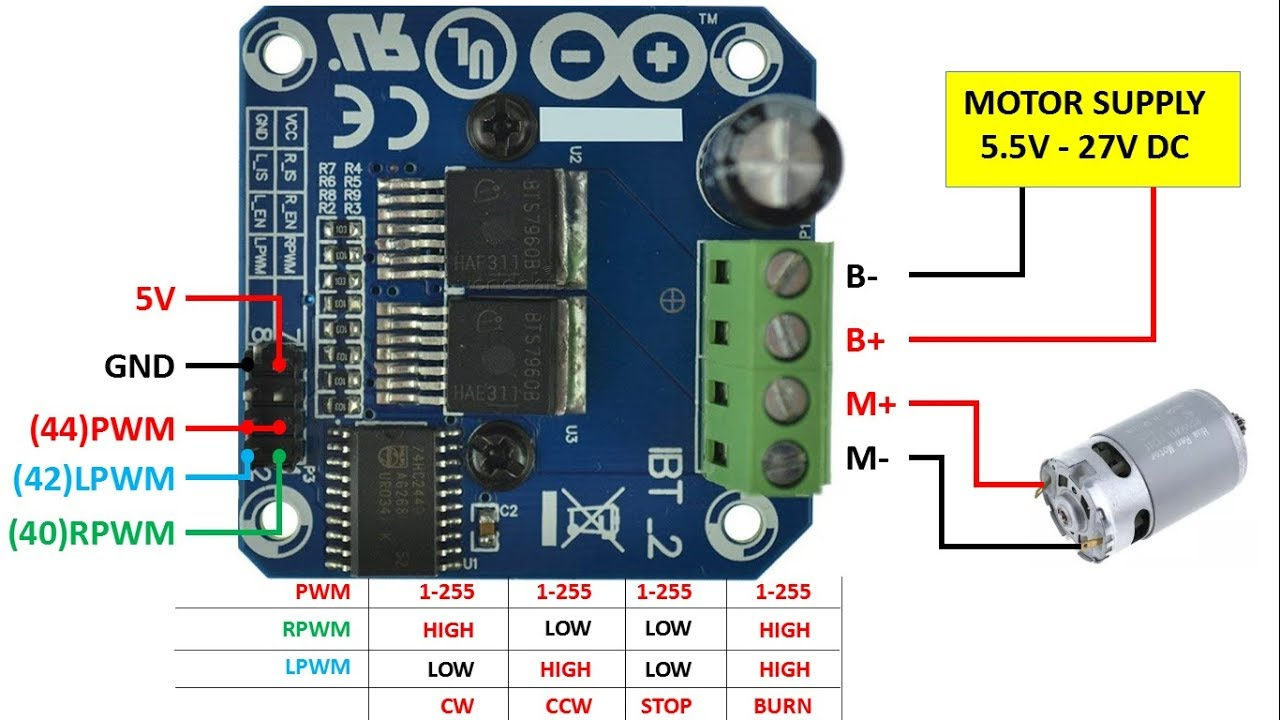
\includegraphics[width=1\textwidth]{IBT-2/TopView.jpg}
	\caption[Driver Motori IBT-2 TopView \& PinOut]{IBT-2 TopView.}
\end{figure}

\noindent
Esso non è un comune Ponte-H integrato, per poter gestire potenze superiori è stato costruito usando 2 Half-Bridge collegati insieme mediante una opportuna logica per ricreare un normale Ponte-H.\\
Questa scheda in particola ha prestazioni interessanti per gli scopi di questa tesi, i principali sono elencati di seguito:\vspace{-8mm}
\begin{center}
	\begin{tabular}[t]{|l r|}
		\hline
		Power Input Voltage:                                     & 6 -- 27 V \\
		Peak current:                                            & 43 A      \\
		Massima Frequenza di PWM:                                & 25 kHz    \\
		Protezione Sovra Tensioni                                &           \\
		Disaccoppiamento Ingresso di Potenza/Logica di controllo &           \\
		\hline
	\end{tabular}
\end{center}
\noindent
Di particolare interesse per l'esperimento è proprio la corrente di picco gestibile:
avendo le dinamiche del sistema tempi inferiori ai 5 secondi, poter reggere correnti di picco così elevate rende
la scheda perfetta per i nostri scopi.

\subsection{Connessione di Controllo}
Il driver permette 2 modalità di funzionamento:
\begin{description}
	\item[Doppio PWM] Modalità operativa che richiede l'uso di 2 PWM\\
	      Ciascun PWM controlla uno dei 2 Half-Bridge, e per evitare di bruciare i driver devono essere controllati singolarmente, il vantaggio di questa configurazione è la possibilità di usare 2 frequenze di controllo diverse.
	\item[Singolo PWM] Modalità operativa classica di un normale Ponte-H\\
	      In questa modalità, la porta nand presente sulla scheda attua la logica di controllo opportuna per governare i 2 Half-Brige come fossero un normale Ponte-H.
\end{description}

\noindent
Per il nostro esperimento si è scelto di usare il collegamento Singolo PWM così da evitare spiacevoli sorprese e avere il PWM di controllo sempre sincronizzato.	

\newpage
\subsection{Benchmark Driver}
Il driver sulla carta à buone prestazioni, ma non sono descritte le sue \nonLinearita, per farle risaltare si sono effettuati 2 esperimenti usando differenti input di controllo:
\begin{enumerate}
	\item \nameref{lst:ondaTriangloare} \\ \vspace{-11mm}
	      \begin{figure}[h]
		      \centering
		      %Todo: Ricampionare l'onda triangolare senza filtro deadzone
		      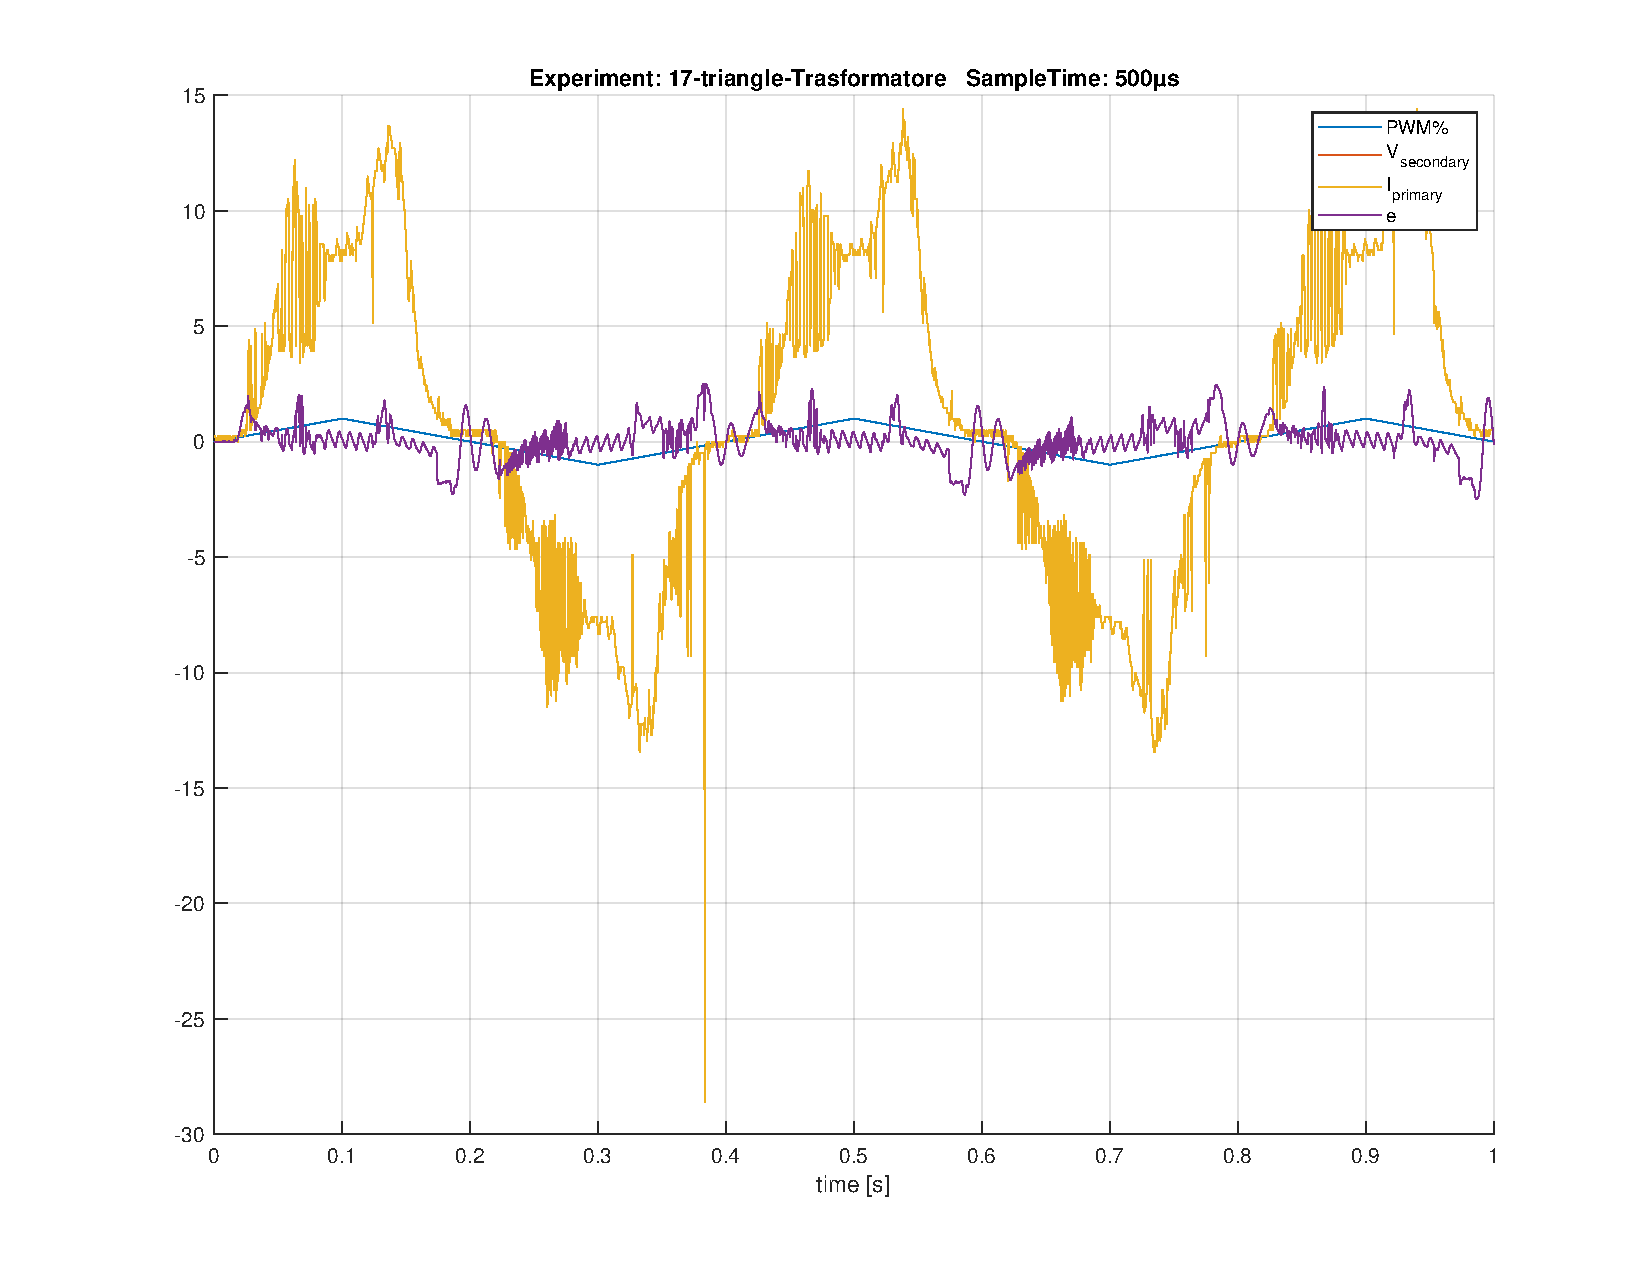
\includegraphics[height=0.5\textheight]{IBT-2/17-triangle-Trasformatore.pdf}
		      \caption[Esperimento con Onda Triangolare]{Onda Triangolare}
	      \end{figure}\vspace{-10mm}
	      \paragraph{Dead-Zone Inferiore} L'onda triangolare si presta bene per far risaltare la problematica della Dead-Zone Inferiore, infatti in tutti gli intorni in cui il segnale passa per 0, è possibile vedere come la corrente non vari minimamente, è però possibile notare che i 2 lati non sono simmetrici tra di loro, questo è facilmente spiegabile dal fatto che il primo ha una condizione iniziale $ \neq $ 0 e di fatto stiamo ancora osservando l'esaurimento del transitorio, la soglia di Dead-Zone Inferiore è quindi calcolata vedendo il primo valore di PWM  per cui il sistema risponde a destra degli 0.      
	      
	      \newpage
	\item \nameref{lst:ondaTrapezoidale} \\
	      \begin{figure}[h]
		      \centering
		      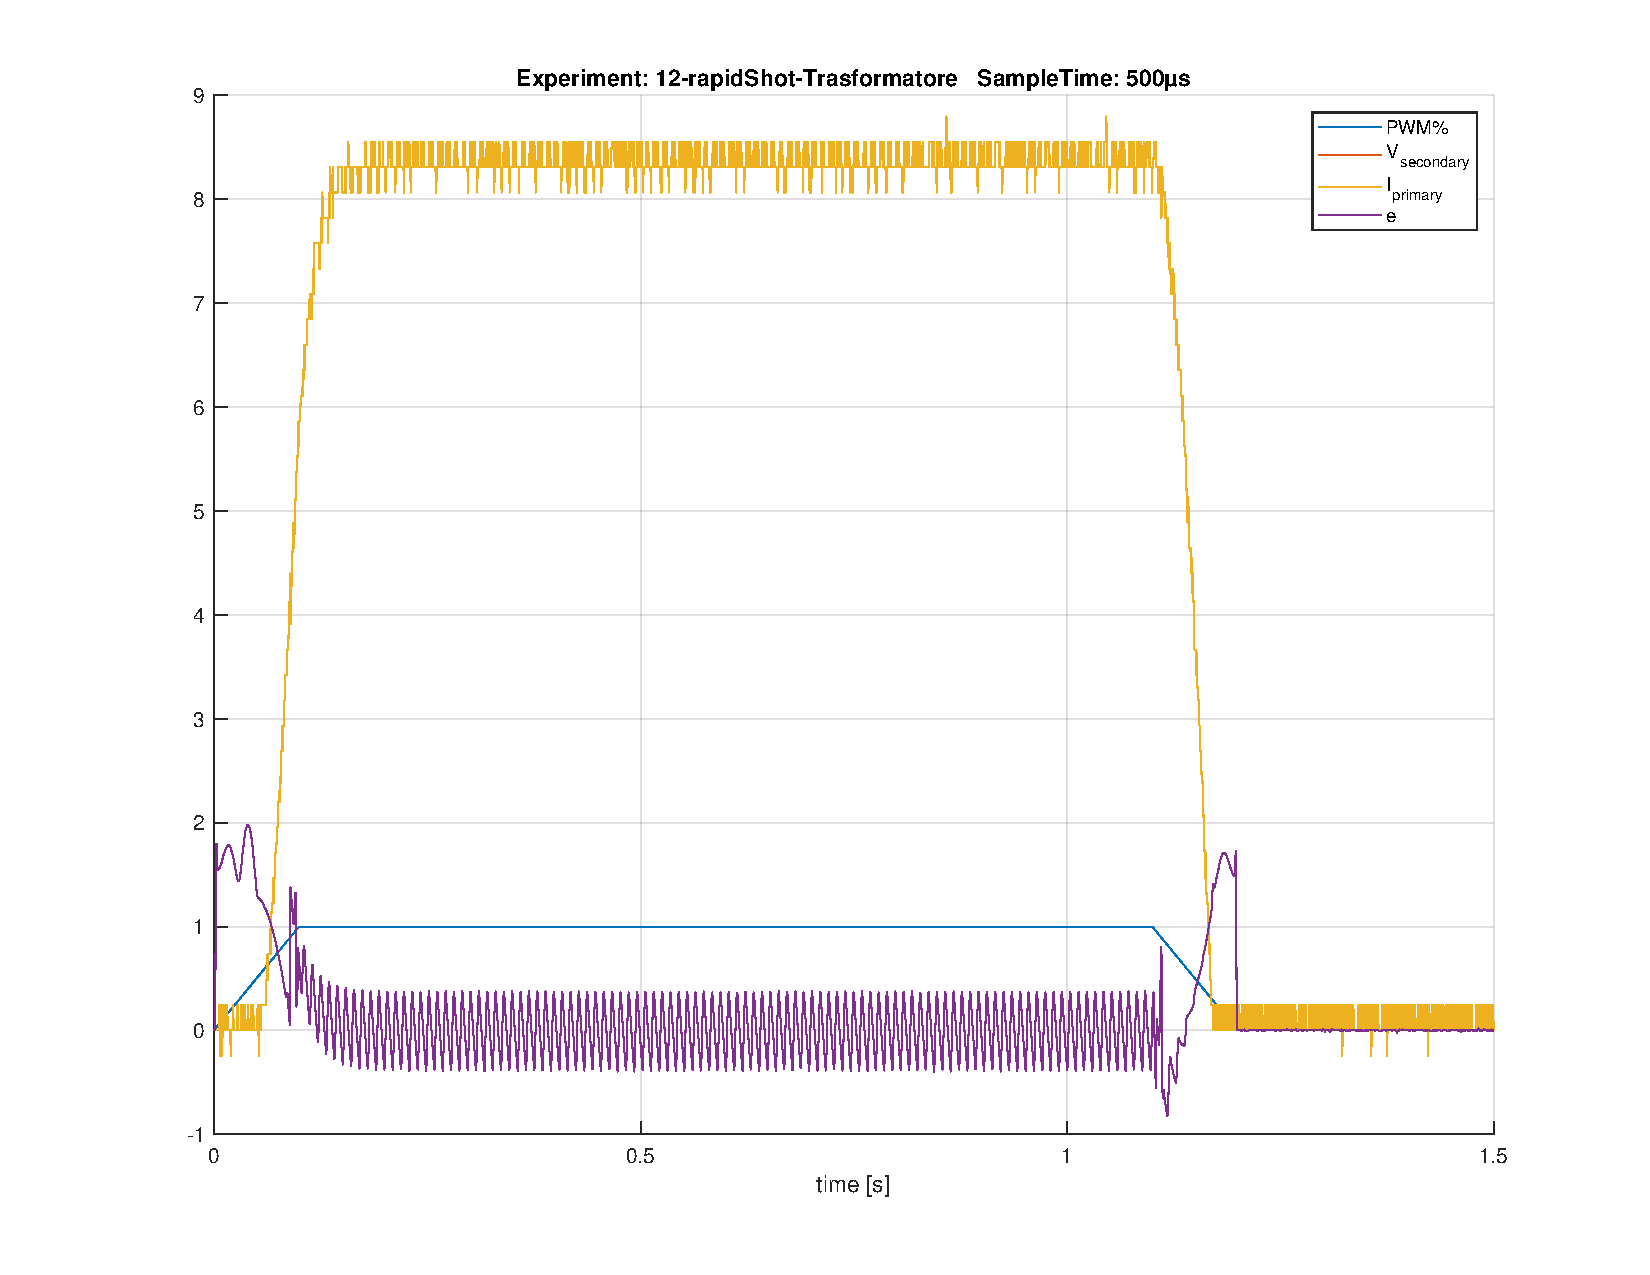
\includegraphics[height=0.5\textheight]{IBT-2/12-rapidShot-Trasformatore.pdf}
		      \caption[Esperimento con Onda Trapezoidale]{Onda Trapezoidale}
	      \end{figure}  \vspace{-10mm}
	      \paragraph{Dead-Zone Superiore} Con questo secondo segnale, si vuole mettere in evidenza il ritardo durante la discesa della rampa, pari a circa 20ms {\small \textit{(guarda 1.1s)}}, questo ritardo è in realtà dovuto da una seconda Dead-Zone presente però ai Duty-Cycle alti del PWM.
	      \vspace{-5mm}
	      \paragraph{Disturbo 50Hz} Essendo in oltre presente un segnale costante per un pò, quando i transitori terminano risulta evidente la presenza della 50hz nel segnale della corrente proveniente dall'alimentatore, questo disturbo è però dovuto alla fonte della corrente, ovvero la 220Vac del laboratorio, il medesimo esperimento realizzato con una batteria non ha disturbi così marcati.
\end{enumerate}
